\subsection{Démarrer les différents services Hadoop:}

\begin{enumerate}
\item \textbf{Vérifié la version de Java:} Avant de poursuivre regardons que java c correctement installer avec la version 8.

Pour cela sur le terminale taper la commande \texttt{java -version}

\begin{figure}[h]
	\centering
    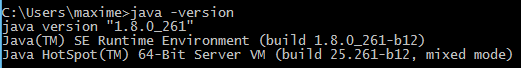
\includegraphics[scale=0.6]{img/part3/3.1}
    \caption{Résultat de la commande}
\end{figure}

\item \textbf{Démarrage des services Hadoop: }

Maintenant, nous allons ouvrir le terminale et accéder au répertoire « \% $HADOOP HOME$ \% \{\}sbin ». Ensuite, nous exécuterons la commande suivante pour démarrer les nœuds Hadoop : \texttt{start-dfs.cmd}
\begin{figure}[h]
	\centering
    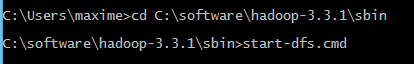
\includegraphics[scale=0.6]{img/part3/3.2}
    \caption{Démarrage des Nœuds Hadoop}
\end{figure}

Deux fenêtres d'invite de commande s'ouvriront (une pour le namenode et une pour le datanode) comme suit:
\begin{figure}[h]
	\centering
    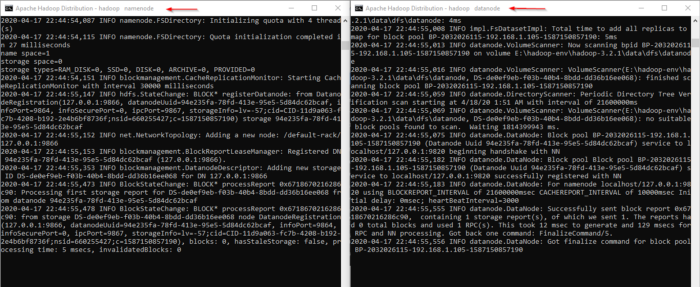
\includegraphics[scale=0.4]{img/part3/3.3}
    \caption{ Fenêtres d'invite de commande des nœuds Hadoop}
\end{figure}

\newpage
Ensuite, nous devons démarrer le service Hadoop Yarn à l'aide de la commande suivante : \texttt{start-yarn.cmd}
\begin{figure}[h]
	\centering
    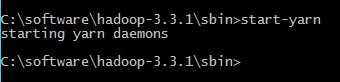
\includegraphics[scale=0.6]{img/part3/3.4}
    \caption{Démarrage des services Hadoop Yarn}
\end{figure}

Deux fenêtres d'invite de commande s'ouvriront (une pour le gestionnaire de ressources et une pour le gestionnaire de nœuds) comme suit :
\begin{figure}[h]
	\centering
    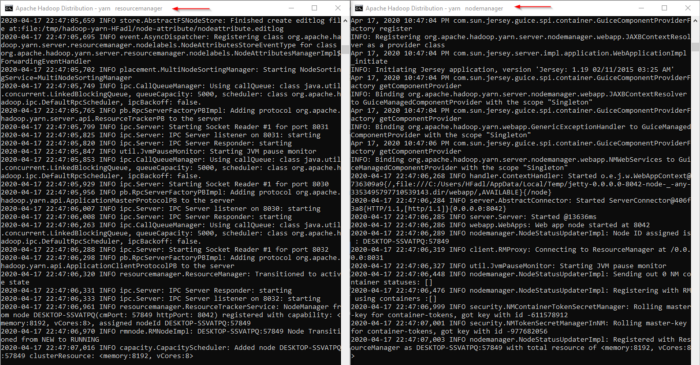
\includegraphics[scale=0.6]{img/part3/3.5}
    \caption{Fenêtres d'invite de commande du gestionnaire de nœuds et du gestionnaire de ressources}
\end{figure}

\end{enumerate}